\scanpage{83}

\deleted{\unsure{approximate} $(\rho_i)(\sigma_i)$ by the systems $(\rho'_i)=(\unsure{\rho_i})$, $(\sigma_i+\varepsilon)$ \inserted{\deleted{$(\sigma'_i)=$}} \illegible{1} of the \unsure{same} \illegible{1} \unsure{for} $k=\unsure{n}$, $\rho'_i,\sigma'_i$ which still satisfy the conditions \unsure{enumerated} \unsure{except} that $\sigma'_{n-1}\ne0$ (by \unsure{taking|setting}}

It therefore suffices, in the \deleted{\unsure{general}}\inserted{\unsure{$\sigma_n=0$|\deleted{$\sigma_n=0$}}} case, \unsure{\deleted{to approximate}|to approximate|\deleted{to associate}} \inserted{to approximate} $(\rho_i)$ $(\sigma_i)$ by an \inserted{admissible system} $(\rho'_i),(\sigma'_i)$ with $\sigma_n>0$, and one will take \deleted{$\unsure{\rho'_i=\rho_i}$}

\deleted{\deleted{\unsure{obviously}} \unsure{the inequality|simply|let us suppose} by some $(\rho'_i),(\sigma'_i)$, with $\sigma'_{n-1}>0$, as one sees by setting $(\rho'_i)=(\rho_i)$, $\sigma_i=\sigma'_i+\varepsilon$ for \deleted{every} $i\leq n-1$, $\sigma'_n=\sigma_n$ (one will have an admissible system, in particular $\prod\rho'_i=\prod\sigma'_i=0$), which brings us back to the case where $\unsure{\sigma}_{n-1}>0$, $\sigma_n=0$. \deleted{\unsure{and whose}}}

\deleted{In this case, if one takes $\sigma'_i=\sigma_i$ for $i\leq n-1$, $\sigma'_n=\sigma_n+\varepsilon$, the system $(\rho_i),(\sigma'_i)$ is admissible, \inserted{for $\varepsilon$ sufficiently small}, except that, in the case where one imposes $\prod\rho_i=\prod\sigma_i$, one will \deleted{\unsure{certainly|perhaps}} not have $\prod\rho_i=\prod\sigma'_i$. But by increasing the zero $\rho_i$ sufficiently little, one obtains a system $(\rho'_i)$ such that one still has \deleted{\unsure{and $\rho$}} $\rho'_1\mathord{-}\,\mathord{-}\rho'_q\leq\sigma'_1\mathord{-}\,\mathord{-}\sigma'_q$ for $q=1,\mathord{-}n$, and \deleted{\unsure{even}}\inserted{by} possible increase of $\rho'_n$ \deleted{\unsure{up to}}\inserted{$\rho''_n$}, \deleted{\unsure{one will obtain|one obtains} $\rho'_1\mathord{.}\,\mathord{-}\rho'_{n-1}\rho''_n=\sigma'_1\mathord{-}\,\mathord{-}\sigma'_n$. \unsure{This system} $\rho'_n=$}}

simply $\rho'_i=\rho_i$, $\sigma'_i=\sigma_i+\varepsilon$.

Let us now prove the lemma. It is well known that a \deleted{every} convex function \deleted{\unsure{$f$}} $\varphi$ on $R^n$ is of the form $\varphi=\operatorname*{Sup}_{\unsure{k|k\in K}}L_k$ where the $L_k$ are \inserted{affine} \uline{linear} \deleted{\uline{\unsure{forms}}}\inserted{functions} on $R^n$ (\unsure{for|this}. follows from the fact that the part of $R^n\times R$ above the graph of $\varphi$ is convex $\unsure{\div}$ by definition of convex functions and \unsure{closed|closed} since $\varphi$ is continuous, --- hence intersection of closed half-spaces, of which one immediately observes
\reversemarginpar
\margin{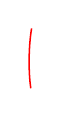
\begin{tikzpicture}[x=1cm,y=1cm]\draw[red,line width=.55pt] (0.02,0.76) .. controls (-0.02,0.52) and (-0.02,0.20) .. (0.01,0);\end{tikzpicture}}
\normalmarginpar
that they \deleted{\unsure{cannot} \unsure{have} as} \textcolor{red}{\uline{\textcolor{black}{\inserted{can} be put}}} \textcolor{red}{\uline{\textcolor{black}{in the form}}} \inserted{of equations} $L_k(t)\geq0$).

Moreover, if $\varphi$ is increasing, one sees \deleted{\unsure{that one} \illegible{2}}\inserted{that} the $L_k$ increas\unsure{ing}, i.e. \deleted{with coefficients} of the form $L_k(t)=\sum_{i=1}^n a_it_i+\unsure{h|b}$, \deleted{\unsure{where the}}\inserted{with} $a_i\geq0$ \inserted{for \deleted{every} $i$}. \deleted{To see this,} : Indeed, if one had $a_i<0$, then \deleted{the function} one

\reversemarginpar
\margin{84}
\normalmarginpar
